% Options for packages loaded elsewhere
\PassOptionsToPackage{unicode}{hyperref}
\PassOptionsToPackage{hyphens}{url}
%
\documentclass[
]{book}
\usepackage{amsmath,amssymb}
\usepackage{lmodern}
\usepackage{iftex}
\ifPDFTeX
  \usepackage[T1]{fontenc}
  \usepackage[utf8]{inputenc}
  \usepackage{textcomp} % provide euro and other symbols
\else % if luatex or xetex
  \usepackage{unicode-math}
  \defaultfontfeatures{Scale=MatchLowercase}
  \defaultfontfeatures[\rmfamily]{Ligatures=TeX,Scale=1}
\fi
% Use upquote if available, for straight quotes in verbatim environments
\IfFileExists{upquote.sty}{\usepackage{upquote}}{}
\IfFileExists{microtype.sty}{% use microtype if available
  \usepackage[]{microtype}
  \UseMicrotypeSet[protrusion]{basicmath} % disable protrusion for tt fonts
}{}
\makeatletter
\@ifundefined{KOMAClassName}{% if non-KOMA class
  \IfFileExists{parskip.sty}{%
    \usepackage{parskip}
  }{% else
    \setlength{\parindent}{0pt}
    \setlength{\parskip}{6pt plus 2pt minus 1pt}}
}{% if KOMA class
  \KOMAoptions{parskip=half}}
\makeatother
\usepackage{xcolor}
\IfFileExists{xurl.sty}{\usepackage{xurl}}{} % add URL line breaks if available
\IfFileExists{bookmark.sty}{\usepackage{bookmark}}{\usepackage{hyperref}}
\hypersetup{
  pdftitle={R Without Statistics},
  pdfauthor={David Keyes},
  hidelinks,
  pdfcreator={LaTeX via pandoc}}
\urlstyle{same} % disable monospaced font for URLs
\usepackage{color}
\usepackage{fancyvrb}
\newcommand{\VerbBar}{|}
\newcommand{\VERB}{\Verb[commandchars=\\\{\}]}
\DefineVerbatimEnvironment{Highlighting}{Verbatim}{commandchars=\\\{\}}
% Add ',fontsize=\small' for more characters per line
\usepackage{framed}
\definecolor{shadecolor}{RGB}{248,248,248}
\newenvironment{Shaded}{\begin{snugshade}}{\end{snugshade}}
\newcommand{\AlertTok}[1]{\textcolor[rgb]{0.94,0.16,0.16}{#1}}
\newcommand{\AnnotationTok}[1]{\textcolor[rgb]{0.56,0.35,0.01}{\textbf{\textit{#1}}}}
\newcommand{\AttributeTok}[1]{\textcolor[rgb]{0.77,0.63,0.00}{#1}}
\newcommand{\BaseNTok}[1]{\textcolor[rgb]{0.00,0.00,0.81}{#1}}
\newcommand{\BuiltInTok}[1]{#1}
\newcommand{\CharTok}[1]{\textcolor[rgb]{0.31,0.60,0.02}{#1}}
\newcommand{\CommentTok}[1]{\textcolor[rgb]{0.56,0.35,0.01}{\textit{#1}}}
\newcommand{\CommentVarTok}[1]{\textcolor[rgb]{0.56,0.35,0.01}{\textbf{\textit{#1}}}}
\newcommand{\ConstantTok}[1]{\textcolor[rgb]{0.00,0.00,0.00}{#1}}
\newcommand{\ControlFlowTok}[1]{\textcolor[rgb]{0.13,0.29,0.53}{\textbf{#1}}}
\newcommand{\DataTypeTok}[1]{\textcolor[rgb]{0.13,0.29,0.53}{#1}}
\newcommand{\DecValTok}[1]{\textcolor[rgb]{0.00,0.00,0.81}{#1}}
\newcommand{\DocumentationTok}[1]{\textcolor[rgb]{0.56,0.35,0.01}{\textbf{\textit{#1}}}}
\newcommand{\ErrorTok}[1]{\textcolor[rgb]{0.64,0.00,0.00}{\textbf{#1}}}
\newcommand{\ExtensionTok}[1]{#1}
\newcommand{\FloatTok}[1]{\textcolor[rgb]{0.00,0.00,0.81}{#1}}
\newcommand{\FunctionTok}[1]{\textcolor[rgb]{0.00,0.00,0.00}{#1}}
\newcommand{\ImportTok}[1]{#1}
\newcommand{\InformationTok}[1]{\textcolor[rgb]{0.56,0.35,0.01}{\textbf{\textit{#1}}}}
\newcommand{\KeywordTok}[1]{\textcolor[rgb]{0.13,0.29,0.53}{\textbf{#1}}}
\newcommand{\NormalTok}[1]{#1}
\newcommand{\OperatorTok}[1]{\textcolor[rgb]{0.81,0.36,0.00}{\textbf{#1}}}
\newcommand{\OtherTok}[1]{\textcolor[rgb]{0.56,0.35,0.01}{#1}}
\newcommand{\PreprocessorTok}[1]{\textcolor[rgb]{0.56,0.35,0.01}{\textit{#1}}}
\newcommand{\RegionMarkerTok}[1]{#1}
\newcommand{\SpecialCharTok}[1]{\textcolor[rgb]{0.00,0.00,0.00}{#1}}
\newcommand{\SpecialStringTok}[1]{\textcolor[rgb]{0.31,0.60,0.02}{#1}}
\newcommand{\StringTok}[1]{\textcolor[rgb]{0.31,0.60,0.02}{#1}}
\newcommand{\VariableTok}[1]{\textcolor[rgb]{0.00,0.00,0.00}{#1}}
\newcommand{\VerbatimStringTok}[1]{\textcolor[rgb]{0.31,0.60,0.02}{#1}}
\newcommand{\WarningTok}[1]{\textcolor[rgb]{0.56,0.35,0.01}{\textbf{\textit{#1}}}}
\usepackage{longtable,booktabs,array}
\usepackage{calc} % for calculating minipage widths
% Correct order of tables after \paragraph or \subparagraph
\usepackage{etoolbox}
\makeatletter
\patchcmd\longtable{\par}{\if@noskipsec\mbox{}\fi\par}{}{}
\makeatother
% Allow footnotes in longtable head/foot
\IfFileExists{footnotehyper.sty}{\usepackage{footnotehyper}}{\usepackage{footnote}}
\makesavenoteenv{longtable}
\usepackage{graphicx}
\makeatletter
\def\maxwidth{\ifdim\Gin@nat@width>\linewidth\linewidth\else\Gin@nat@width\fi}
\def\maxheight{\ifdim\Gin@nat@height>\textheight\textheight\else\Gin@nat@height\fi}
\makeatother
% Scale images if necessary, so that they will not overflow the page
% margins by default, and it is still possible to overwrite the defaults
% using explicit options in \includegraphics[width, height, ...]{}
\setkeys{Gin}{width=\maxwidth,height=\maxheight,keepaspectratio}
% Set default figure placement to htbp
\makeatletter
\def\fps@figure{htbp}
\makeatother
\setlength{\emergencystretch}{3em} % prevent overfull lines
\providecommand{\tightlist}{%
  \setlength{\itemsep}{0pt}\setlength{\parskip}{0pt}}
\setcounter{secnumdepth}{-\maxdimen} % remove section numbering
\ifLuaTeX
  \usepackage{selnolig}  % disable illegal ligatures
\fi
\usepackage[]{natbib}
\bibliographystyle{apalike}

\title{R Without Statistics}
\author{David Keyes}
\date{}

\begin{document}
\maketitle

{
\setcounter{tocdepth}{1}
\tableofcontents
}
\hypertarget{about-the-book}{%
\chapter*{About the Book}\label{about-the-book}}
\addcontentsline{toc}{chapter}{About the Book}

This is the in-progress version of \emph{R Without Statistics}, a forthcoming book from \href{https://www.nostarch.com/}{No Starch Press}.

Since R was invented in 1993, it has become a widely used programming language for statistical analysis. From academia to the tech world and beyond, R is used for a wide range of statistical analysis.

R's ubiquity in the world of statistics leads many to assume that it is only useful to those who do complex statistical work. But as R has grown in popularity, the number of ways it can be used has grown as well. Today, R is used for:

\begin{itemize}
\item
  Data visualization
\item
  Map making
\item
  Sharing results through reports, slides, and websites
\item
  Automating processes
\item
  And much more!
\end{itemize}

The idea that R is only for statistical analysis is outdated and inaccurate. But, without a single book that demonstrates the power of R for non-statistical purposes, this perception persists.

\textbf{Enter R Without Statistics.}

R Without Statistics will show ways that R can be used beyond complex statistical analysis. Readers will learn about a range of uses for R, many of which they have likely never even considered.

Each chapter will, using a consistent format, cover one novel way of using R.

\begin{enumerate}
\def\labelenumi{\arabic{enumi}.}
\item
  Readers will first be introduced to an R user who has done something novel and learn how using R in this way transformed their work.
\item
  Following this, there will be code samples that demonstrate exactly how the R user did the thing they are being profiled for.
\item
  Finally, there will be a summary, with lessons learned from this novel way of using R.
\end{enumerate}

Written by David Keyes, Founder and CEO of~\href{https://rfortherestofus.com/}{R for the Rest of Us}, R Without Statistics will be published by \href{https://nostarch.com/}{No Starch Press}.

\begin{Shaded}
\begin{Highlighting}[]
\FunctionTok{library}\NormalTok{(tidyverse)}
\CommentTok{\#\textgreater{} {-}{-} Attaching packages {-}{-}{-}{-}{-}{-}{-}{-}{-}{-}{-}{-}{-}{-}{-}{-}{-}{-}{-} tidyverse 1.3.1 {-}{-}}
\CommentTok{\#\textgreater{} v ggplot2 3.3.5     v purrr   0.3.4}
\CommentTok{\#\textgreater{} v tibble  3.1.6     v dplyr   1.0.8}
\CommentTok{\#\textgreater{} v tidyr   1.2.0     v stringr 1.4.0}
\CommentTok{\#\textgreater{} v readr   2.1.2     v forcats 0.5.1}
\CommentTok{\#\textgreater{} {-}{-} Conflicts {-}{-}{-}{-}{-}{-}{-}{-}{-}{-}{-}{-}{-}{-}{-}{-}{-}{-}{-}{-}{-}{-} tidyverse\_conflicts() {-}{-}}
\CommentTok{\#\textgreater{} x dplyr::filter() masks stats::filter()}
\CommentTok{\#\textgreater{} x dplyr::lag()    masks stats::lag()}
\FunctionTok{library}\NormalTok{(readxl)}
\FunctionTok{library}\NormalTok{(janitor)}
\CommentTok{\#\textgreater{} }
\CommentTok{\#\textgreater{} Attaching package: \textquotesingle{}janitor\textquotesingle{}}
\CommentTok{\#\textgreater{} The following objects are masked from \textquotesingle{}package:stats\textquotesingle{}:}
\CommentTok{\#\textgreater{} }
\CommentTok{\#\textgreater{}     chisq.test, fisher.test}
\FunctionTok{library}\NormalTok{(knitr)}
\FunctionTok{library}\NormalTok{(tweetrmd)}
\end{Highlighting}
\end{Shaded}

\hypertarget{part-introduction}{%
\part*{Introduction}\label{part-introduction}}
\addcontentsline{toc}{part}{Introduction}

\hypertarget{why-r-without-statistics}{%
\chapter*{Why R Without Statistics?}\label{why-r-without-statistics}}
\addcontentsline{toc}{chapter}{Why R Without Statistics?}

\hypertarget{how-new-zealand-used-r-to-fight-covid}{%
\section*{How New Zealand Used R to Fight COVID}\label{how-new-zealand-used-r-to-fight-covid}}
\addcontentsline{toc}{section}{How New Zealand Used R to Fight COVID}

TODO

\hypertarget{how-i-came-to-use-r}{%
\section*{How I Came to Use R}\label{how-i-came-to-use-r}}
\addcontentsline{toc}{section}{How I Came to Use R}

My own relationship with R goes back to 2016. At the time, I was a consultant, helping non-profits, government agencies, and educational institutions to measure the effectiveness of their work is (a field known as \href{https://www.cdc.gov/evaluation/index.htm}{program evaluation}). A lot of my work involved conducting surveys, analyzing the resulting the data, and sharing the results with clients.

The work itself was fine, but the tools I was using to do it were getting on my nerves. Well, one tool really: Excel.

Now look, this is not a place for an anti-Excel rant. Excel is a fine tool that has empowered millions to work with data in ways they would never have been able to otherwise.

But, for me, Excel was tedious. The amount of pointing and clicking I had to do when working with the amount of data I had got old fast. Each time I would conduct a survey, I'd know that it would yield an avalanche of data and that my wrists would end up exhausted from hours of pointing and clicking.

No matter what I did, analyzing data and creating charts in Excel just involved a lot of repetitive pointing and clicking. Kind of like this:

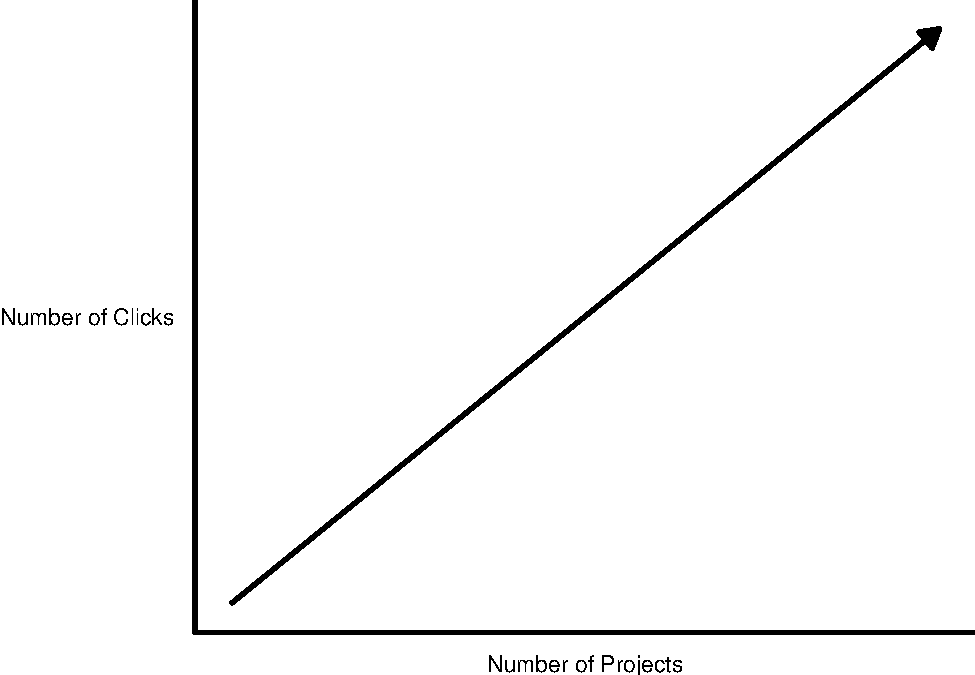
\includegraphics{introduction_files/figure-latex/unnamed-chunk-2-1.pdf}

Endless pointing and clicking was just one problem I faced using Excel. Annoying though it was, it didn't affect the quality of my work. Or so I thought until I recalled a project I had worked on a few years earlier.

In this project, I was looking at which school districts in the state of Oregon have \href{https://oregonstate.app.box.com/s/83g5sjdm88xgqdxfze0ri7qo4uff5sj7}{outdoor education programs known as Outdoor School}. As part of this project, I had to download data on all school districts throughout Oregon, filter to only include relevant districts with fifth or sixth graders (the ages Outdoor School takes place), and then merge this with data that I collected as part of a survey I conducted.

I did the work in Excel, using a lot of (you guessed it!) pointing and clicking. The problem came when I was almost done with the project. I've blocked the details from my memory (as I've done with most things Excel-related), but what I do recall is that not being 100\% certain I had done my filtering and joining correctly. And, to make it worse, I had no way to check my work. Why? Because all my pointing and clicking was ephemeral, gone in the ether as soon as I had completed it.

I finished the Outdoor School project and submitted my report. I think the work I did was \emph{probably} accurate, but maybe it wasn't?

Now, you may be reading this thinking: why didn't you write down the steps you used in Excel so you could retrace them later? Sure, I could (and should) have done that. But let's be honest: most of us don't.

The reality is, we're human. We all make mistakes. And without a straightforward way to audit your work (and keeping a list of all of your Excel points and clicks in a separate document is not, in my view, straightforward), mistakes will happen. If you've used Excel to work with data, I guarantee you've made a mistake, just like me.

The good news is that it's ok. There's a solution. And that solution is R.

If I were to redo that project on Outdoor School with R, here's what I'd do differently. Rather than watching points and clicks disappear into the ether, I'd write code that would serve as a record of everything I did. This code would:

Download data on all school districts:

\begin{Shaded}
\begin{Highlighting}[]
\CommentTok{\# Download the data directly from the Oregon Department of Education website}
\FunctionTok{download.file}\NormalTok{(}\AttributeTok{url =} \StringTok{"https://www.oregon.gov/ode/educator{-}resources/assessment/Documents/TestResults2019/pagr\_schools\_ela\_tot\_raceethnicity\_1819.xlsx"}\NormalTok{,}
              \AttributeTok{destfile =} \StringTok{"data/pagr\_schools\_ela\_tot\_raceethnicity\_1819.xlsx"}\NormalTok{)}

\CommentTok{\# Import the downloaded data and use the \textasciigrave{}clean\_names()\textasciigrave{} function to make the variable names easy to work with}
\NormalTok{oregon\_schools }\OtherTok{\textless{}{-}} \FunctionTok{read\_excel}\NormalTok{(}\StringTok{"data/pagr\_schools\_ela\_tot\_raceethnicity\_1819.xlsx"}\NormalTok{) }\SpecialCharTok{\%\textgreater{}\%} 
  \FunctionTok{clean\_names}\NormalTok{()}
\end{Highlighting}
\end{Shaded}

Filter to only include districts with fifth or sixth graders:

\begin{Shaded}
\begin{Highlighting}[]
\CommentTok{\# Start with the oregon\_schools data from above}
\NormalTok{oregon\_schools\_fifth\_sixth\_grade }\OtherTok{\textless{}{-}}\NormalTok{ oregon\_schools }\SpecialCharTok{\%\textgreater{}\%} 
  
  \CommentTok{\# Only keep schools with fifth or sixth graders}
  \FunctionTok{filter}\NormalTok{(grade\_level }\SpecialCharTok{==} \StringTok{"Grade 5"} \SpecialCharTok{|}\NormalTok{ grade\_level }\SpecialCharTok{==} \StringTok{"Grade 6"}\NormalTok{) }\SpecialCharTok{\%\textgreater{}\%} 
  
  \CommentTok{\# Only keep the variables we need}
  \FunctionTok{select}\NormalTok{(district\_id}\SpecialCharTok{:}\NormalTok{school) }\SpecialCharTok{\%\textgreater{}\%} 
  
  \CommentTok{\# There are multiple observations of the same school, just keep one of each}
  \FunctionTok{distinct}\NormalTok{()}
\end{Highlighting}
\end{Shaded}

Join the filtered data on school districts with my survey data:

\begin{Shaded}
\begin{Highlighting}[]
\CommentTok{\# Use the school\_id variable to join the survey data with the oregon\_schools\_fifth\_sixth\_grade from above }
\FunctionTok{left\_join}\NormalTok{(survey\_data, oregon\_schools\_fifth\_sixth\_grade,}
          \AttributeTok{by =} \StringTok{"school\_id"}\NormalTok{)}
\end{Highlighting}
\end{Shaded}

Code can be scary. Having to write code is one of the reasons many people never learn R. But code is just a list of things you want to do to your data. It may be written in a hard-to-parse syntax (though it gets easier over time), but it's just a set of steps. The same steps that we should write out when we're working in Excel, but never do. Rather than having a separate document with my steps written down (the one that never gets written), I can see my steps in my code. See that line that says filter. Guess what it's doing? Yep, it's filtering!

If I had done things this way when working on the Outdoor School project, I could have looked back at any point to make sure what I thought was happening to my data was in fact happening. That nagging sensation I had near the end of the project that I may have made a mistake in one of my early points or clicks? It never would come up because I could just review my code to make sure it did what I thought it did. And if it didn't, I could rewrite and rerun my code to get updated results.

Using R won't mean you'll never make mistakes again (trust me, you will). But it will mean that you can easily spot your mistakes, make changes, and fix any issues.

I started learning R to avoid tedious pointing and clicking. But what I found was that R improved my work in ways I never expected. It's not just that my wrists are less tired. I now have more confidence that my work is accurate.

\begin{center}\rule{0.5\linewidth}{0.5pt}\end{center}

I used to feel ashamed about the way I use R.

I use R, a tool for statistical analysis, but I don't use it for complex statistical analysis. I don't do machine learning. I don't know what a random forest is. I've never even run a regression in R.

\href{https://rfortherestofus.com/2018/12/descriptive-stats-r/}{The only statistics I do in R are descriptive statistics}. Counts, sums, averages: these are the statistics that I do in R.

For a long time, I felt like I wasn't a ``real'' R user. Real R users, in my mind, used R for hardcore stats. I ``only'' used R for descriptive stats.

I sometimes felt like I was using a souped up sports car to drive 20 miles an hour to the grocery store. What was the point in using a high-powered machine like R to do ``simple'' things?

Eventually, I realized that this framing misses the point. \href{https://rss.onlinelibrary.wiley.com/doi/10.1111/j.1740-9713.2018.01169.x}{R started out as a tool created by statisticians for other statisticians}. But, over a quarter century since its creation, R can do much more than statistical analysis.

My own use of R is an example of this. I think of my work with R in three buckets:

\textbf{Illuminate} through data visualization: making graphs, maps, and tables that look good and share results effectively.

TODO: Add examples

\textbf{Communicate} by doing reporting with RMarkdown: moving away from the inefficiency and error-prone workflow of using multiple tools to create reports by instead doing it all in the one tool that I think of as \href{https://rfortherestofus.com/2019/03/r-killer-feature-rmarkdown/}{R's killer feature}.

TODO: Add some image

\textbf{Automate} tedious practices: Remember my Excel-burdened wrists? Since I moved to R I've found so many ways to automate tedious practices, from gathering data directly from the U.S. Census Bureau to pulling survey results in from Qualtrics and more.

TODO: Add some image

The main reason I've come to accept that my way of using R is as valid as anyone else's has come through realizing that more ``sophisticated'' R users are doing many of the same things I am. Sure, they may also be doing statistical analyses that I am not, but everyone who uses R needs to illuminate, communicate, and automate.

Canadian statistician Sharla Gelfand has \href{https://twitter.com/sharlagelfand/status/1135962094938009601}{talked about how they used R to automate an annual report on nursing registration exams in Ontario}. Sharla told me in 2019 that, despite being a statistician, \href{https://rfortherestofus.com/2019/09/my-r-journey-sharla-gelfand/}{the most statistical thing they did was calculating a median}.

Take a look at the R community on Twitter (where users congregate under the \#rstats hashtag). What gets people most excited is not the latest complex statistical analysis. \href{https://twitter.com/dgkeyes/status/1479473689225695234}{It's tips and tricks on the foundational work that everyone who uses R needs to do}.

\href{https://twitter.com/CedScherer/status/1220843943224578050}{Things like making illuminating data visualizations} as part of the \href{https://github.com/rfordatascience/tidytuesday}{Tidy Tuesday project}.

\href{https://twitter.com/spcanelon/status/1424932510065209348}{Or video tutorials on how to communicate through effective presentations using R}.

\href{https://twitter.com/WeAreRLadies/status/1228049014601342976}{Or love letters to the \texttt{clean\_names()} function from the \texttt{janitor} package, which automates the process of making messy variable names easy to work with in R}.

No matter what else you do in R, you have to \textbf{illuminate} your findings and \textbf{communicate} your results. And, the more you use R, the more you'll find yourself wanting to \textbf{automate} things you used to do manually (your wrists will thank you).

I realize now that the things that I use R for \emph{are} the things that everyone uses R for. R was created for statistics. But today people are just as likely to use R without statistics.

Ten years ago, if you had told me I'd be writing a book on R, I'd have laughed. As someone with an extremely non-quantitative background (I did a PhD in anthropology) who never used R in graduate school, I never thought I'd be in a position to teach people about R. But here we find ourselves. And I'm excited to be your guide on this journey through the ways you can use R without statistics.

If I only used R for the things I thought ``real'' R users used it for, I wouldn't be writing this book. But, instead of slogging away in the world of complex statistical analysis, far outside of my area of expertise, I have found a place for myself in the world of R. Expanding my conception of what R can do has enabled me to get more out of this tool.

And here's the thing: if I, a qualitatively-trained anthropologist whose most complex statistical use for R is calculating averages, can find value in R, so can you. No matter what your background or what you think about R right now, using R without statistics can transform how you work in the future.

\hypertarget{how-this-book-works}{%
\section*{How This Book Works}\label{how-this-book-works}}
\addcontentsline{toc}{section}{How This Book Works}

This book shows the many ways that people use R without statistics. It's not comprehensive (trust me, there are many ways people use R not covered here). But I hope the ideas inspire you to think about learning to use R (if you're not yet an R user) or (if you are already on board the R train) learning to use R in ways you hadn't previously considered.

Each chapter focuses on one novel use of R. You'll begin by learning about a user or users who have transformed their work using R. You'll learn about a problem they had and how R helped them to solve it.We'll dive into their code, analyzing it line by line in order to help you understand how they used R. Each chapter will conclude with a short summary, offering lessons you can take from this novel way of using R.

I've tried to choose topics for each chapter that are relevant to a broad audience. Things like data visualization, report generation, and creating your own functions are things that anyone, no matter what you use R for, will find valuable.

There are some great topics that I thought to include but were just too narrow in their focus (for example, \href{https://blog.djnavarro.net/posts/2021-10-19_rtistry-posts/}{the world of generative art made with R}. If, at any point while you're reading this book, you think, ``why didn't David include X topic,'' please know that X might be a great topic, but I can only cover so much. The fact that you're able to come up with other ideas for things that R can do is a) fantastic and b) a further display of R's versatility. I eagerly await your follow-up book highlighting the myriad other things R can do that I am unable to cover in this book!

\hypertarget{a-favor-to-ask}{%
\section*{A Favor to Ask}\label{a-favor-to-ask}}
\addcontentsline{toc}{section}{A Favor to Ask}

Pedants of the world (as one of you, I come in peace), I have a favor to ask.

This book is called R Without Statistics. But it's not meant to be taken literally.

Of course it's true that if you're making a graph you're using statistics. So, before you start typing an angry email to me, please know that R Without Statistics is a mindset rather than a literal statement.

We're all using R with statistics already. Let's also learn to use R without statistics.

\hypertarget{part-illuminate}{%
\part*{Illuminate}\label{part-illuminate}}
\addcontentsline{toc}{part}{Illuminate}

\hypertarget{use-general-principles-of-high-quality-data-viz-in-r}{%
\chapter*{Use General Principles of High-Quality Data Viz in R}\label{use-general-principles-of-high-quality-data-viz-in-r}}
\addcontentsline{toc}{chapter}{Use General Principles of High-Quality Data Viz in R}

\hypertarget{develop-a-custom-theme-to-keep-your-data-viz-consistent}{%
\chapter*{Develop a Custom Theme to Keep Your Data Viz Consistent}\label{develop-a-custom-theme-to-keep-your-data-viz-consistent}}
\addcontentsline{toc}{chapter}{Develop a Custom Theme to Keep Your Data Viz Consistent}

\hypertarget{r-is-a-full-fledged-map-making-tool}{%
\chapter*{R is a Full-Fledged Map-Making Tool}\label{r-is-a-full-fledged-map-making-tool}}
\addcontentsline{toc}{chapter}{R is a Full-Fledged Map-Making Tool}

\hypertarget{make-tables-that-look-good-and-share-results-effectively}{%
\chapter*{Make Tables That Look Good and Share Results Effectively}\label{make-tables-that-look-good-and-share-results-effectively}}
\addcontentsline{toc}{chapter}{Make Tables That Look Good and Share Results Effectively}

\hypertarget{part-communicate}{%
\part*{Communicate}\label{part-communicate}}
\addcontentsline{toc}{part}{Communicate}

\hypertarget{use-rmarkdown-to-communicate-accurately-and-efficiently}{%
\chapter*{Use RMarkdown to Communicate Accurately and Efficiently}\label{use-rmarkdown-to-communicate-accurately-and-efficiently}}
\addcontentsline{toc}{chapter}{Use RMarkdown to Communicate Accurately and Efficiently}

\hypertarget{use-rmarkdown-to-instantly-generate-hundreds-of-reports}{%
\chapter*{Use RMarkdown to Instantly Generate Hundreds of Reports}\label{use-rmarkdown-to-instantly-generate-hundreds-of-reports}}
\addcontentsline{toc}{chapter}{Use RMarkdown to Instantly Generate Hundreds of Reports}

\url{https://urban-institute.medium.com/using-r-markdown-to-track-and-publish-state-data-d1291bfa1ec0}

\hypertarget{create-beautiful-presentations-with-rmarkdown}{%
\chapter*{Create Beautiful Presentations with RMarkdown}\label{create-beautiful-presentations-with-rmarkdown}}
\addcontentsline{toc}{chapter}{Create Beautiful Presentations with RMarkdown}

\hypertarget{make-websites-to-share-results-online}{%
\chapter*{Make Websites to Share Results Online}\label{make-websites-to-share-results-online}}
\addcontentsline{toc}{chapter}{Make Websites to Share Results Online}

\hypertarget{part-automate}{%
\part*{Automate}\label{part-automate}}
\addcontentsline{toc}{part}{Automate}

\hypertarget{access-up-to-date-census-data-with-the-tidycensus-package}{%
\chapter*{\texorpdfstring{Access Up to Date Census Data with the \texttt{tidycensus} Package}{Access Up to Date Census Data with the tidycensus Package}}\label{access-up-to-date-census-data-with-the-tidycensus-package}}
\addcontentsline{toc}{chapter}{Access Up to Date Census Data with the \texttt{tidycensus} Package}

\hypertarget{pull-in-survey-results-as-soon-as-they-come-in}{%
\chapter*{Pull in Survey Results as Soon as They Come In}\label{pull-in-survey-results-as-soon-as-they-come-in}}
\addcontentsline{toc}{chapter}{Pull in Survey Results as Soon as They Come In}

\hypertarget{stop-copying-and-pasting-code-by-creating-your-own-functions}{%
\chapter*{Stop Copying and Pasting Code by Creating Your Own Functions}\label{stop-copying-and-pasting-code-by-creating-your-own-functions}}
\addcontentsline{toc}{chapter}{Stop Copying and Pasting Code by Creating Your Own Functions}

\hypertarget{bundle-your-functions-together-in-your-own-r-package}{%
\chapter*{Bundle Your Functions Together in Your Own R Package}\label{bundle-your-functions-together-in-your-own-r-package}}
\addcontentsline{toc}{chapter}{Bundle Your Functions Together in Your Own R Package}

\hypertarget{part-conclusion}{%
\part*{Conclusion}\label{part-conclusion}}
\addcontentsline{toc}{part}{Conclusion}

\hypertarget{come-for-the-data-stay-for-the-community}{%
\chapter*{Come for the Data, Stay for the Community}\label{come-for-the-data-stay-for-the-community}}
\addcontentsline{toc}{chapter}{Come for the Data, Stay for the Community}

\end{document}
